\section{DnsRR}\label{sec:dnsrr}

\begin{figure}
\begin{center}
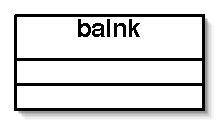
\includegraphics[width=0.4\textwidth]{figs/blank}
\end{center}
\caption{}
\label{fig:dnsrr}
\end{figure}

This section describes the component, which is described by Figure~\ref{fig:dnsrr}.  

This represents an RR of any type for which we do not have a specific implementation. It handles the high-level functions of a DNS RR packet.

\subsection{Methods}

{\bf Public Methods}
\begin{itemize}
\item parse(): Takes a wire representation of a DNS packet and parses it into an RR. This is a factory method, and will return an object inheriting from DnsRR depending on the type of the RR.
\item type(): Returns the numeric type of the RR. A list of symbolic constants for common types is included.
\item rdata\_valid(): Returns true if the RDATA is of a valid format (which depends on the underlying RR type).
\item set\_rdata(): Set the RDATA section to a bag of bytes.
\end{itemize}

{\bf Private Methods}
\begin{itemize}
\item factory(): Static factory method that returns a new RR of a numeric type, used by parse\_question\_rr() and parse\_normal\_rr().
\item parse\_question\_rr(): Parse an RR from the question section, returns an RR of the proper type if no error occurs.
\item parse\_normal\_rr(): Parse an RR from any section other than the questions section. Returns RR of the proper type if no error occurs.
\end{itemize}

\subsection{Member Variables}

\begin{itemize}
\item m\_init: True if the object has been init.
\item m\_name: DnsName object representing the name of the packet.
\item m\_type: Numeric type of the RR.
\item m\_class: RR class (as defined by RFC1035).
\item m\_ttl: TTL of RR (-1 if question RR).
\item m\_rdata: Binary RDATA.
\item m\_rdlen: Length of RDATA.
\end{itemize}
